\documentclass[final,hyperref={pdfpagelabels=false},xcolor=svgnames]{beamer}

\mode<presentation>
  {
  \usetheme{Boadilla}
  %\usetheme{Frankfurt}
  }
 \usepackage[orientation=landscape,size=E,scale=1.5,debug]{beamerposter}

%	\usepackage{rotating}

  %%%%%%%%%%%%%%%%%%%%%%%%%%%%%%%%%%%%%%%%%%%%%%%%%%%%%%%%%%%%%%%%%%%%%%%%%%%%%%%%%5
  \title[]{\VeryHuge \textbf{ CodeMeta: A Rosetta Stone for Software Metadata }}
  \author{Carl Boettiger}
  \institute{Environmental Science, Policy, and Management, University of California, Berkeley}
  \usecolortheme[named=DarkBlue]{structure} 

\setbeamertemplate{background canvas}{\includegraphics[width=\paperwidth,height=\paperheight]{../public/img/rosetta-table.jpg}}

%%%%%%%% PANDOC Boilerplate header

\usepackage{lmodern}
\usepackage{amssymb,amsmath}
\usepackage{ifxetex,ifluatex}
\usepackage{fixltx2e} % provides \textsubscript
\ifnum 0\ifxetex 1\fi\ifluatex 1\fi=0 % if pdftex
  \usepackage[T1]{fontenc}
  \usepackage[utf8]{inputenc}
\else % if luatex or xelatex
  \ifxetex
    \usepackage{mathspec}
  \else
    \usepackage{fontspec}
  \fi
  \defaultfontfeatures{Ligatures=TeX,Scale=MatchLowercase}
\fi
% use upquote if available, for straight quotes in verbatim environments
\IfFileExists{upquote.sty}{\usepackage{upquote}}{}
% use microtype if available
\IfFileExists{microtype.sty}{%
\usepackage{microtype}
\UseMicrotypeSet[protrusion]{basicmath} % disable protrusion for tt fonts
}{}
\usepackage{hyperref}
\hypersetup{unicode=true,
            pdftitle={Untitled},
            pdfborder={0 0 0},
            breaklinks=true}
\urlstyle{same}  % don't use monospace font for urls
\usepackage{color}
\usepackage{fancyvrb}
\usepackage{listings}
\newcommand{\VerbBar}{|}
\newcommand{\VERB}{\Verb[commandchars=\\\{\}]}
\usepackage{graphicx,grffile}
\makeatletter
\def\maxwidth{\ifdim\Gin@nat@width>\linewidth\linewidth\else\Gin@nat@width\fi}
\def\maxheight{\ifdim\Gin@nat@height>\textheight\textheight\else\Gin@nat@height\fi}
\makeatother
% Scale images if necessary, so that they will not overflow the page
% margins by default, and it is still possible to overwrite the defaults
% using explicit options in \includegraphics[width, height, ...]{}
\setkeys{Gin}{width=\maxwidth,height=\maxheight,keepaspectratio}
\IfFileExists{parskip.sty}{%
\usepackage{parskip}
}{% else
\setlength{\parindent}{0pt}
\setlength{\parskip}{6pt plus 2pt minus 1pt}
}
\setlength{\emergencystretch}{3em}  % prevent overfull lines
\providecommand{\tightlist}{%
  \setlength{\itemsep}{0pt}\setlength{\parskip}{0pt}}
\setcounter{secnumdepth}{0}
% Redefines (sub)paragraphs to behave more like sections
\ifx\paragraph\undefined\else
\let\oldparagraph\paragraph
\renewcommand{\paragraph}[1]{\oldparagraph{#1}\mbox{}}
\fi
\ifx\subparagraph\undefined\else
\let\oldsubparagraph\subparagraph
\renewcommand{\subparagraph}[1]{\oldsubparagraph{#1}\mbox{}}
\fi

%%%%%%%%%%%%%%%%%%%%%%%%%%%%%%%%%%%%%%%%%%%%%%%%%%%%%%%%%%%%%%%%%%%%%%%%%%%%%%%%%5
  \begin{document}
  \begin{frame}[t,fragile] 
%  \maketitle

          \frametitle{\VeryHuge{\textbf{ Codemeta: A Rosetta Stone for Software Metadata } }\\
          \LARGE{\hspace{1cm} EArly-concept Grants for Exploratory Research (EAGER) \\
          \hspace{1cm} Carl Boettiger, UC Berkeley}}
\vspace{3cm}

%%%%%%%%%%%%%%%% Two top columns %%%%%%%%%%%%%%%

\begin{columns}[t] % LEFT COLUMN 
  \begin{column}{.30\paperwidth}
 
        {\LARGE Abstract } \\
  
        Research relies heavily on scientific software, and a large and growing
        fraction of researchers are engaged in developing software as part of
        their own research
        (\href{http://dx.doi.org/10.1109/SECSE.2009.5069155}{Hannay et al 2009}).
        Despite this, \emph{infrastructure to support the preservation,
        discovery, reuse, and attribution of software} lags substantially behind
        that of other research products such as journal articles and research
        data. This lag is driven not so much by a lack of technology as it is by
        a lack of unity: existing mechanisms to archive, document, index, share,
        discover, and cite software contributions are heterogeneous among both
        disciplines and archives and rarely meet best practices
        (\href{http://dx.doi.org/10.1002/asi.23538}{Howison 2015}).
        Fortunately, a rapidly growing movement to improve preservation,
        discovery, reuse and attribution of academic software is now underway: a
        recent \href{http://softwarediscoveryindex.org}{NIH report}, conferences
        and working groups of \href{https://www.force11.org/}{Force11},
        \href{http://wssspe.researchcomputing.org.uk/}{WSSSPE} \&
        \href{http://www.software.ac.uk/}{Software Sustainability Institute},
        and the rising adoption of repositories like
        \href{https://github.com}{GitHub}, \href{https://zenodo.org}{Zenodo},
        \href{https://figshare.com}{figshare} \&
        \href{https://www.dataone.org}{DataONE} by academic software developers.
        Codemeta is a distributed open source project to improve how these resources
        can talk to each other.\\
        
        \vspace{1cm}
  
        {\LARGE Example JSON-LD}

	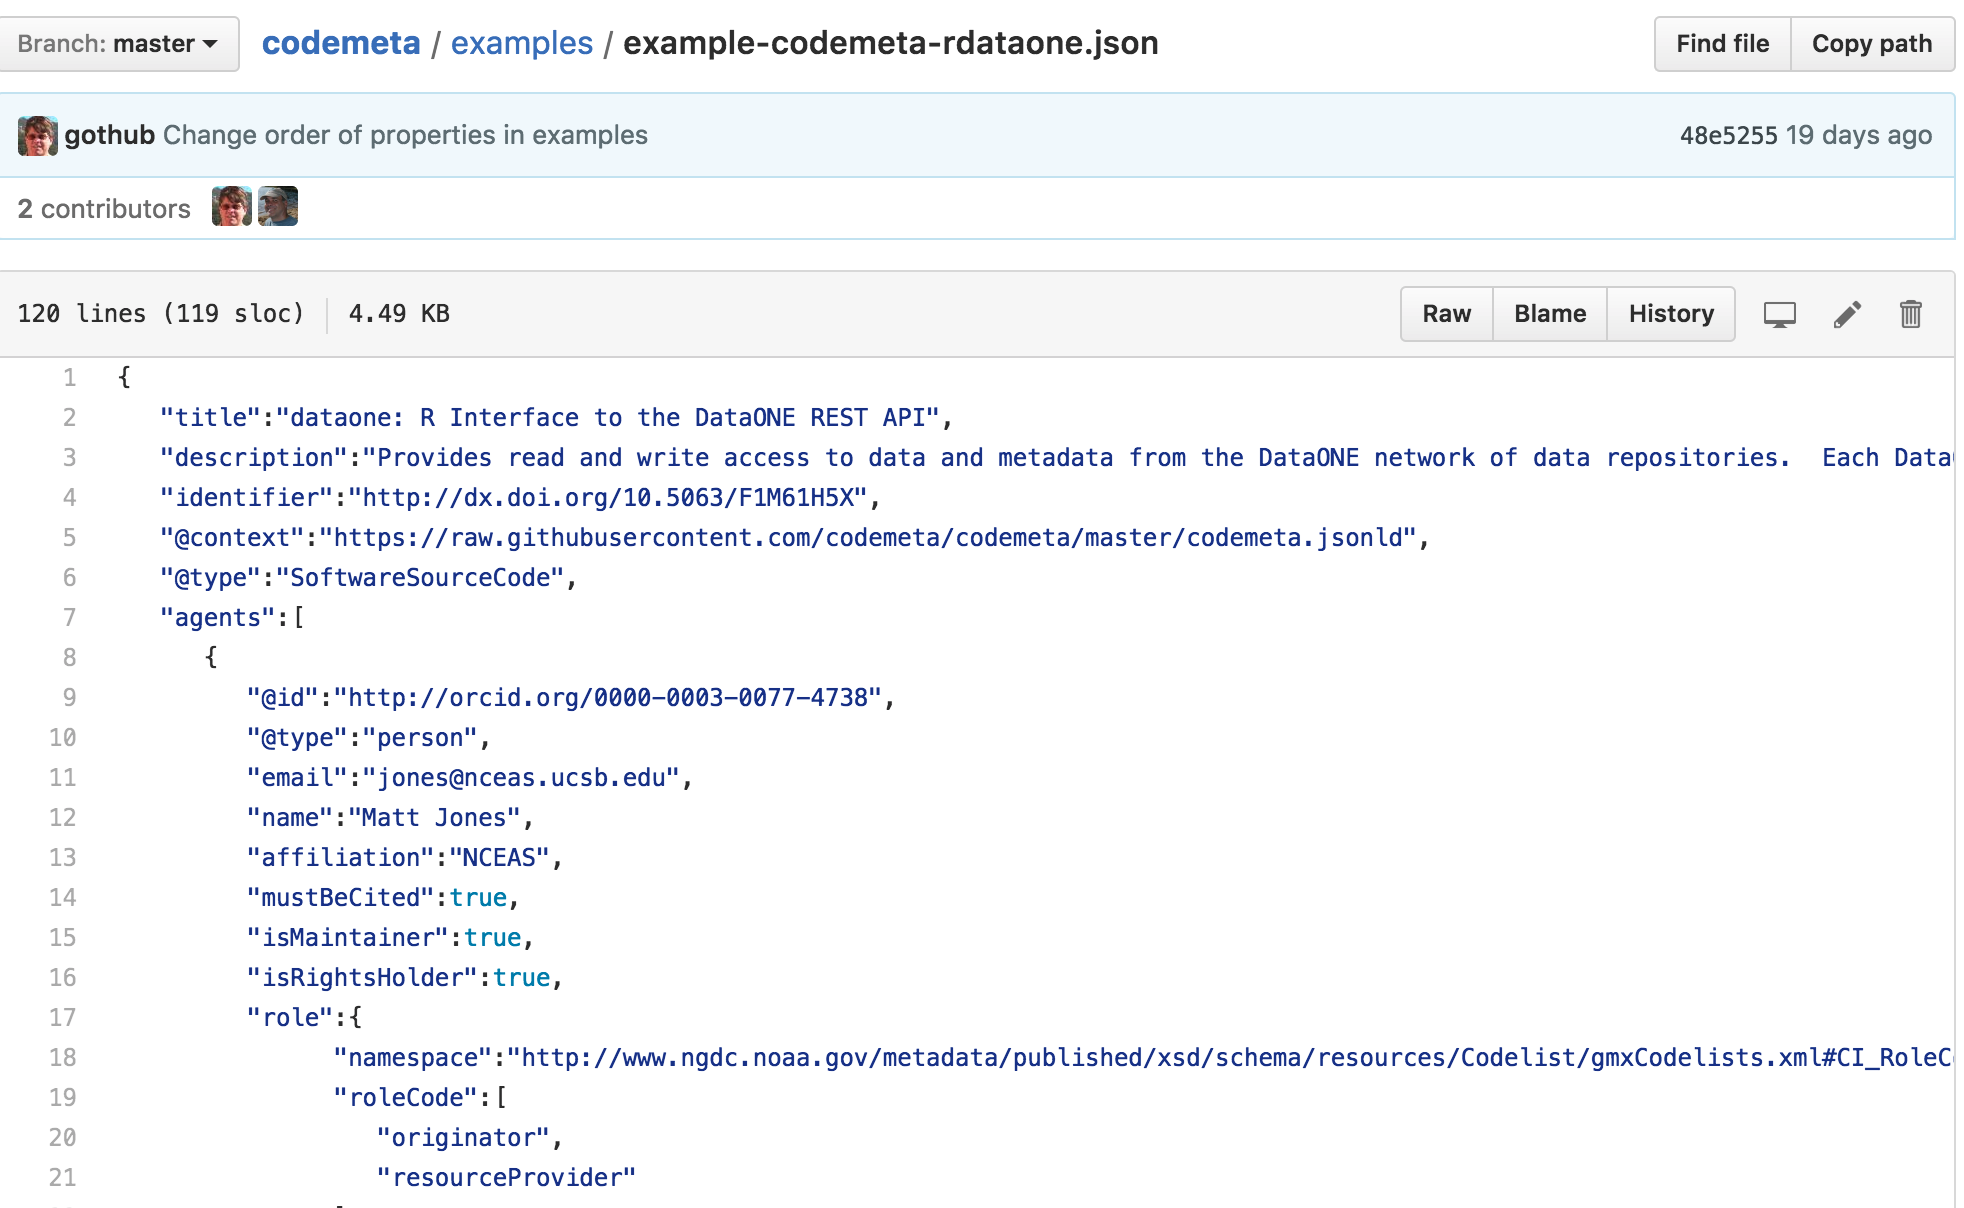
\includegraphics[width=.30\paperwidth]{../public/img/codemeta-json.png}

  \end{column}
%%%%%%%%%%%%%% CENTER-LEFT COLUMN %%%%%%%%%%%%%%%%%%%%
  \begin{column}{.33\paperwidth} 
  {\LARGE A Metadata CrossWalk}

  18 contributors met in Portland, OR on April 15-17, 2016
  to agree on a draft crosswalk between major software metadata schema.
  

  \vspace{2.5cm}

  {\LARGE Schemas in Crosswalk }

  DataCite, OntoSoft, Zenodo, GitHub, Figshare, Software Ontology,
  Software Discovery Index, Dublin Core, R Package Description,
  Debian Package Metadata, Python Distutils (PyPI), Trove Software
  Map, Perl Module Description (CPAN::Meta), JavaScript package
  descption (npm), Java (Maven), Octave, Ruby Gem, ASCL, Schema.org

  \vspace{2.5cm}


  {\LARGE A JSON-LD Context for Software Metadata }

  \vspace{1cm}
  
\includegraphics[width=30cm]{../public/img/doi.png}
  \vspace{1cm}

  \begin{itemize}
          \item A linked-data representation of codemeta concepts
          \item Basic types from Schema.org, also Dublin Core and XSD
          \item 26 new terms introduced in \texttt{codemeta} namespace
  \end{itemize}


  \vspace{5cm}
  {\LARGE Project Deliverables}\\
  \vspace{1cm}
  \textbf{Project Website}: \href{https://codemeta.github.io}{codemeta.github.io} \\
  \vspace{1cm}
  \textbf{JSON-LD Context file}: \href{https://github.com/codemeta/codemeta/codemeta.jsonld}{github.com/codemeta/codemeta/codemeta.jsonld} \\
  \vspace{1cm}
  \textbf{Crosswalk Table}: \href{https://github.com/codemeta/codemeta/crosswalk.csv}{github.com/codemeta/codemeta/crosswalk.csv} \\
  \vspace{1cm}
  \textbf{\texttt{codemeta.json}} examples: \href{https://github.com/codemeta/codemeta/examples}{github.com/codemeta/codemeta/examples}

  \vspace{1cm}
  { \LARGE Coming soon} \\

  Utilities for automatically generating \texttt{codemeta.json} for common software package types (e.g. R packages)

  Zenodo parsing of \texttt{codemeta.json} into Zenodo metadata and on to DataCite records.

  Partner organizations extend metadata representation



  \end{column}
%%%%  RIGHT COLUMN
  \begin{column}{.33\paperwidth}
        {\LARGE Organizations} \\
        
\includegraphics[width=10cm]{../public/img/nsf.png}\hspace{1cm}	
         
\includegraphics[width=10cm]{../public/img/datacite.png}\hspace{1cm}		
         
\includegraphics[width=10cm]{../public/img/github.png}	

         
\includegraphics[width=10cm]{../public/img/figshare.png}\hspace{1cm}		
         
\includegraphics[width=10cm]{../public/img/dataone.png}\hspace{1cm}		
         
\includegraphics[width=10cm]{../public/img/zenodo.jpg}	
         
         \vspace{5cm}
    \begin{columns}
      \begin{column}{.10\paperwidth}
              %        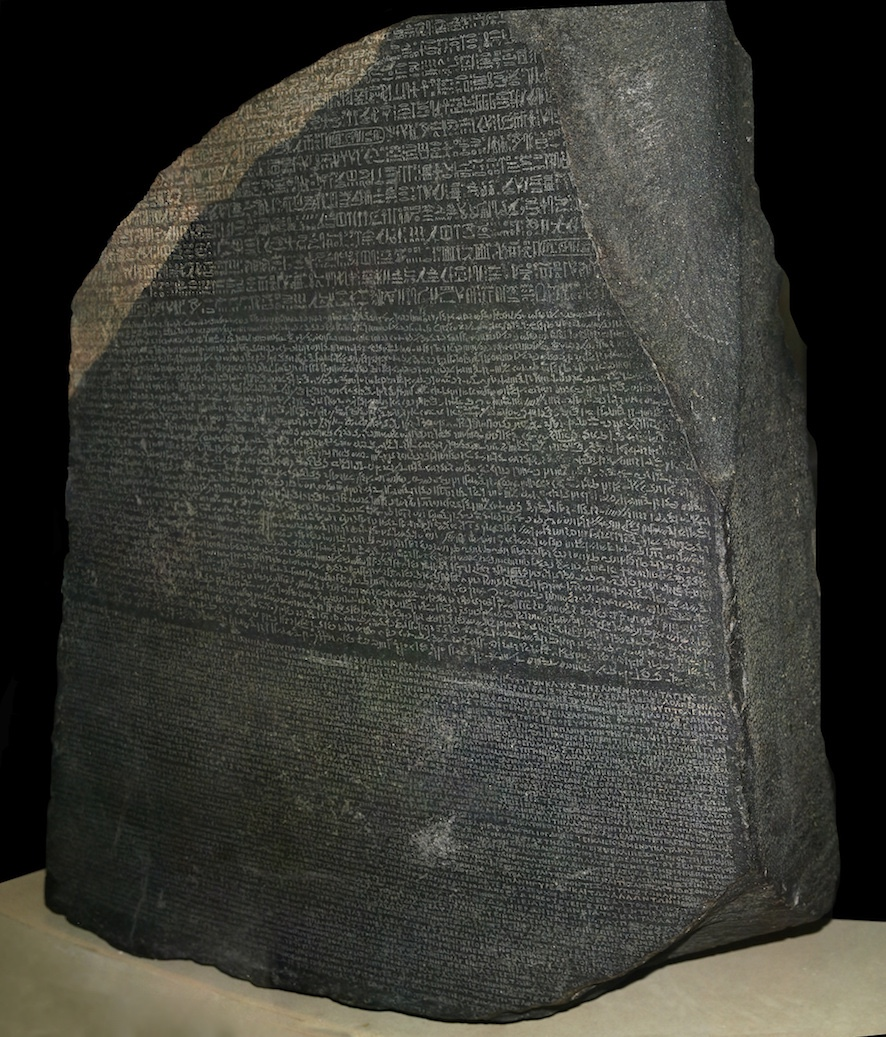
\includegraphics[width=.15\paperwidth]{../public/img/rosetta.jpg} \\ {\tiny CC-BY-SA, Hans Hillewaert}
      \end{column}      
      \begin{column}{.20\paperwidth}
          {\LARGE Workshop Participants} \\
        \begin{itemize}
        \item \href{http://carlboettiger.info}{Carl Boettiger}, UC Berkeley
        \item \href{https://twitter.com/metamattj}{Matt Jones}, NCEAS
        \item \href{http://www.arfon.org/}{Arfon Smith}, GitHub
        \item \href{http://www.isi.edu/~gil/}{Yolanda Gil}, USC ISI
        \item \href{https://twitter.com/mfenner}{Martin Fenner}, DataCite
        \item \href{https://github.com/krzysztof}{Krzysztof Nowak}, Zenodo
        \item \href{https://twitter.com/markhahnel?lang=en}{Mark Hahnel}, figshare
        \item \href{https://twitter.com/abbycabs}{Abby Mayes}, Mozilla Science Lab
        \item \href{http://lukecoy.github.io/}{Luke Coy}, RIT \& MSL
        \item \href{http://kyleniemeyer.com/}{Kyle Niemeyer}, Oregon State
        \item \href{https://twitter.com/asclnet}{Alice Allen}, ASCL
        \item \href{http://scholar.harvard.edu/mercecrosas}{Mercè Crosas}, Harvard, IQSS
        \item \href{https://knowledgeinfrastructures.gseis.ucla.edu/?page_id=62\#Sands}{Ashley Sands}, UCLA
        \item \href{https://twitter.com/npch}{Neil Chue Hong} SSI
        \item \href{https://github.com/sbpcs59}{Peter Slaughter}, NCEAS
        \item \href{https://www.datacite.org/news/datacite-appoints-patricia-cruse-executive-director.html}{Patricia Cruse}, DataCite
        \item \href{http://danielskatz.org/}{Dan Katz}, NCSA
        \item \href{http://www.manchester.ac.uk/research/Carole.goble/}{Carole Goble}, University of Manchester
        \end{itemize}
      \end{column}
    \end{columns}

	See more contributors at
	\href{https://github.com/codemeta/codemeta/graphs/contributors}{github.com/codemeta/codemeta/graphs/contributors}
	and
	\href{https://github.com/codemeta/codemeta/network/members}{github.com/codemeta/codemeta/network/members}
  \end{column}
\end{columns}
\end{frame}
\end{document}

%% Fontsize commands
	%      \tiny
	%      \scriptsize
	%     \footnotesize
	%     \normalsize
	%      \large 
	%      \Large
	 %     \LARGE
	%      \veryHuge
	%      \VeryHuge
	 %     \VERYHuge

